\subsection{Projekt Postaci}
Postaci zostały utworzone przy pomocy strony \url{https://www.mixamo.com}. Wybraliśmy modele, w których przeważają ciemne kolory, a ich charakteryzacja współgra z mrocznym klimatem otoczenia. 
Następnie do każdej postaci zostały dopasowane animacje, które mogliśmy wykorzystać podczas procesu implementacji.
\begin{figure}[H]
	\center
	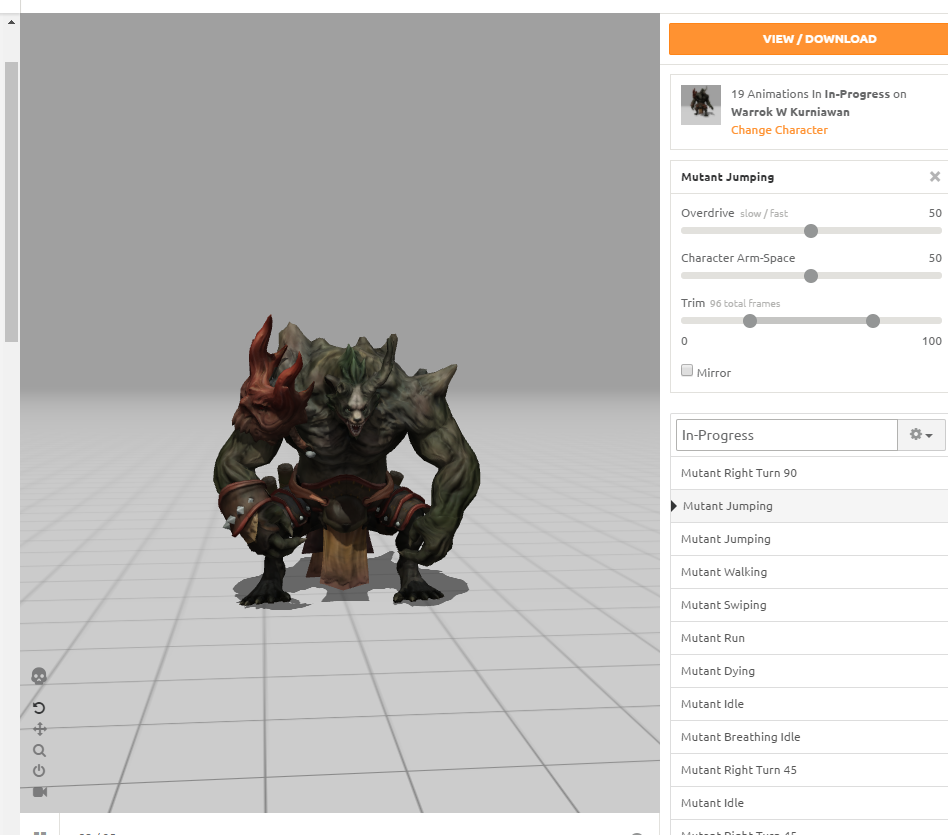
\includegraphics[width=8cm]{mixamo.png}
	\caption{Projekt głównego przeciwnika}
\end{figure}
Ostatnim krokiem było wybranie szczegółów takich jak ilość klatek na sekundę (FPS) z jaką mają być wyświetlane animacje. 
Po wykonaniu powyższych czynności pakiet postaci mógł zostać pobrany, a następnie dołączony do projektu. 